\documentclass{report}
\usepackage{ugentstyle}


\begin{document}

\maketitle{Examen Compilers 14 juni 2019}
%\tableofcontents

\part{Closed Book}
\section*{Question 1}
\begin{enumerate}
    \item Give the transfer functions and dataflow equations for \textit{available expressions}.

    \begin{table}[ht]
        \centering
        \begin{tabular}{|l| l| l|}
            \hline
            Statement s & gen[s] & kill[s] \\
            \hline
             & & \\[1ex]
            $t \leftarrow b \oplus c$ & & \\
            & & \\[1ex]
            \hline
            & & \\[1ex]
            $t \leftarrow M[b]$ & & \\
            & & \\[1ex]
            \hline
            & & \\[1ex]
            $M[a] \leftarrow b$ & & \\
            & & \\[1ex]
            \hline
            & & \\[1ex]
            $f(a_1, ..., a_n)$ & & \\
            & & \\[1ex]
            \hline
            & & \\[1ex]
            $t \leftarrow f(a_1, ..., a_n)$ & & \\
            & & \\[1ex]
            \hline
        \end{tabular}
    \end{table}
    
    $$in[n] = \qquad\qquad\qquad\qquad\qquad\qquad\qquad\qquad\qquad\qquad out[n] = $$

    \item Data flow can be pro
\end{enumerate}
\section*{Question 2}
Consider following code:
\begin{figure}[ht]
    \centering
    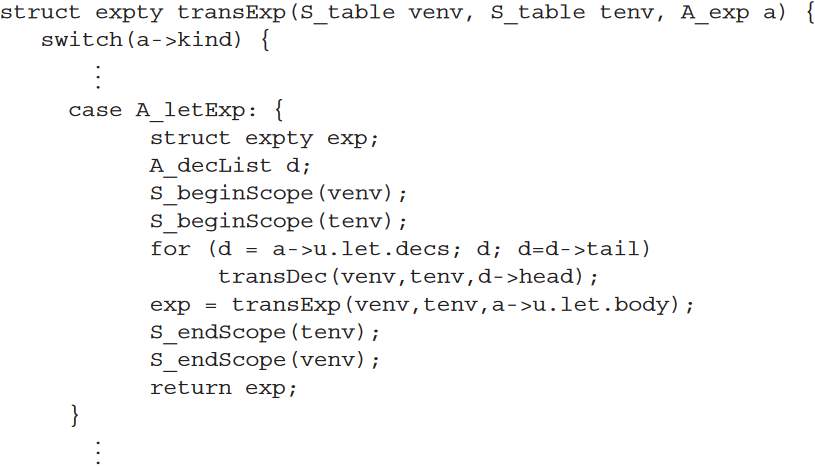
\includegraphics[width=0.73\textwidth]{symboltable}
\end{figure}
It shows two facts about how symbol tables can be implemented. Which facts?

\newpage
\section*{Question 3}
\begin{enumerate}
    \item Which feature(s) should a programming language offer in order to make static links useful.
    \item Explain how static links can be implemented, not neccesarily on an architecture which supports static links.
\end{enumerate}

\section*{Question 4}
\begin{enumerate}
    \item Give the definition of a basic block.
    \item What is the difference between a graph of basic blocks and a trace of basic blocks?
\end{enumerate}

\section*{Question 5}
\todo{iets over componenten met twee register mode}

\section*{Question 6}
Consider the following graph:
\begin{figure}[ht]
    \centering
    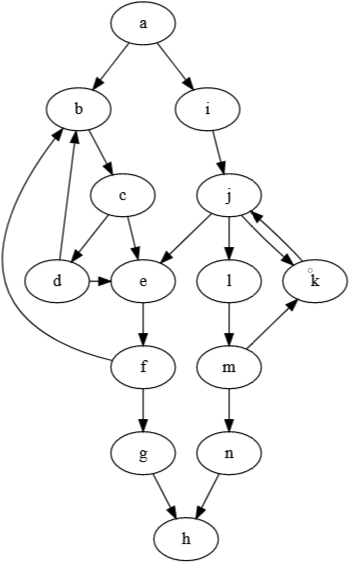
\includegraphics[width=0.4\textwidth]{cfg}
\end{figure}
\begin{enumerate}
    \item Mark the headers of each natural loop in this graph.
    \item Add preheaders in this graph for eventual optimizations.
    \item Fill in the table below, which indicates different relationships between nodes:
    \begin{itemize}
        \item[] P indicates that $x$ (in column) is post-dominated by $y$ (in row).
        \item[] D indicates that $x$ dominates $y$.
        \item[] I indicates that $x$ is the immediate dominator of $y$.
        \item[] df indicates that $x$ is in the dominance frontier of $y$. 
    \end{itemize}
    Some cells have been filled, as an example.

    \begin{table}[ht]
        \centering
        \begin{tabular}{| l || l  | l  | l  | l  | l  | l  | l  | l  | l  | l  | l  | l  | l  | l |}
            \hline
              & a & b & c & d & e & f & g & h & i & j & k & l & m & n \\
            \hline
            a &   &   &   &   &   &   &   & P &   &   &   &   &   &   \\
            \hline
            c &   & I  &   &   &   &   &   &   &   &   &   &   &   &   \\
            \hline
            e & D  &   &   &   &   &   &   &   &   &   &   &   &   &   \\
            \hline
            i &   &   &   &   & df  &   &   &   &   &   &   &   &   &   \\
            \hline
            j &   &   &   &   &   &   &   &   &   &   &   &   &   &   \\
            \hline
        \end{tabular}
    \end{table}
\end{enumerate}


\section*{Question 10}
Given the following grammar:
\begin{align*}
    S &\rightarrow E \\
    E &\rightarrow i\\
    E &\rightarrow i(E)\\
    E &\rightarrow E + 1\\
\end{align*}
\begin{enumerate}
    \item Give the first and follow sets.
    \item Give the production rules for the remaining states (3, 5 and 7) in the following SLR state table:
    \begin{figure}[ht]
		\centering
		\begin{tikzpicture}[state/.style={rectangle, draw, inner sep = 2mm}]
		\node (1) [state] {
            $\begin{aligned}
                S \mapsto& .E \\
                E \mapsto& .i \\
                E \mapsto& .i(E) \\
                E \mapsto& .E + i
            \end{aligned}$
        };

        \node (2) [state, above= 1cm of 1] {
            $\begin{aligned}
                S \mapsto& E. \\
                E \mapsto& E. + i
            \end{aligned}$
        };

        \node (3) [state, right= 1cm of 1] {
            $\begin{aligned}
                \qquad\qquad\qquad\\
                \qquad\qquad\qquad\\
                \qquad\qquad\qquad\\
            \end{aligned}$
        };

        \node (4) [state, right= 1cm of 2] {
            $\begin{aligned}
                E \mapsto& E +. i
            \end{aligned}$
        };

        \node (5) [state, right= 1cm of 3] {
            $\begin{aligned}
                \qquad\qquad\qquad\\
                \qquad\qquad\qquad\\
                \qquad\qquad\qquad\\
            \end{aligned}$
        };
        \node (6) [state, right= 1cm of 4] {
            $\begin{aligned}
                E \mapsto& E + i.
            \end{aligned}$
        };

        \node (7) [state, right= 1cm of 5] {
            $\begin{aligned}
                \qquad\qquad\qquad\\
                \qquad\qquad\qquad\\
                \qquad\qquad\qquad\\
            \end{aligned}$
        };

        \node (8) [state, right= 1cm of 6] {
            $\begin{aligned}
                E \mapsto E + .i
            \end{aligned}$
        };
        \node (9) [state, right= 1cm of 7] {
            $\begin{aligned}
                E \mapsto i(E).
            \end{aligned}$
        };
		
		
		\draw [->] (1) -- node[xshift=0.25cm] {E} (2);
        \draw [->] (1) -- node[yshift=0.25cm] {i} (3);   
        \draw [->] (2) -- node[yshift=0.25cm] {+} (4);   
        \draw [->] (4) -- node[yshift=0.25cm] {i} (6);   
        \draw [->] ([yshift=10pt] 3.east) -- node[yshift=0.25cm] {(} ([yshift=10pt] 5.west);    
        \draw [->] ([yshift=-10pt] 5.west) -- node[yshift=-0.25cm] {i} ([yshift=-10pt] 3.east);    
        \draw [->] (5) -- node[yshift=0.25cm] {E} (7); 
        \draw [->] (7) -- node[xshift=0.25cm] {+} (8);     
        \draw [->] (8) -- node[yshift=0.25cm] {i} (6);  
		\draw [->] (7) -- node[yshift=0.25cm] {i} (9);  
        \node (label1) [anchor=north east, inner sep = 1pt] at (1.north east) {\textbf{1.}};
        \node (label2) [anchor=north east, inner sep = 1pt] at (2.north east) {\textbf{2.}};
        \node (label3) [anchor=north east, inner sep = 1pt] at (3.north east) {\textbf{3.}};
        \node (label5) [anchor=north east, inner sep = 1pt] at (5.north east) {\textbf{5.}};
        \node (label6) [anchor=north east, inner sep = 1pt] at (6.north east) {\textbf{6.}};
        \node (label7) [anchor=north east, inner sep = 1pt] at (7.north east) {\textbf{7.}};
        \node (label8) [anchor=north east, inner sep = 1pt] at (8.north east) {\textbf{8.}};
        \node (label9) [anchor=north east, inner sep = 1pt] at (9.north east) {\textbf{9.}};
		\end{tikzpicture}
    \end{figure}
    \item Are there shift-reduce conflicts in state 3? Explain.
\end{enumerate}
\part{Open Book}
\section*{Question 1 (5pt)}
The following table gives an interference graph. Cells marked $x$ mean an non-move reated interferences between vertices. Cells marked $m$ are move-related. Registers 1-4 are precolored, while registers A-E have to be assigned a color. Color this graph with coalescing and using 5 registers. Show only the phases used in the following format:
\begin{lstlisting}
simplify A
coalesce A and 1 (George) int 1A    # the names are in alphabetical order
freeze A
spill A
select A
\end{lstlisting}
\begin{table}[ht]
    \centering
    \begin{tabular}{c | c c c c c c c c c}
            & 1 & 2 & 3 & 4 & A & B & C & D & E \\
            \hline
        A   & x &   & x &mx &   &   & x & x &  x \\
        B   & x &   & m & x &   &   & x & x & m \\
        C   & m & x & x &   & x & x &   & x & x \\
        D   & x & x & x & x & x & x & x &   & x \\
        E   &   & x  &  &  &  x & m  & x & x &   \\
    \end{tabular}
\end{table}

\section*{Question 2 (5pt)}

\end{document}
